\documentclass[11pt,a4paper]{article}

\usepackage{microtype}
\usepackage{graphicx}
\usepackage{listings}
\usepackage{siunitx}
\usepackage{hyperref}
\usepackage{float}

\title{MPI Assignment}
\author{Jan van der Lugt}
\date{}

\begin{document}
\maketitle

\section{Introduction}
The report discusses my implementation of a parallel all-pairs shortest path (ASP) algorithm based on the famous Floyd-Warshall algorithm.

Section 2 explain will go through changes that were made to the sequential program, while section 3 will report performance results, including a speedup graph. Section 4 will answer various questions from the KIC.

\section{Implementation}
The Floyd-Warshall ASP algorithm is very well and easily parallelizeable: every row has to be transmitted only once from its owner to all other processes, after which everyone uses this row to update distance values for their share of the distance table. This mimics the sequential execution, which can be seen as a special case of the parallel version with only one worker who is responsible for the entire table.

The calculation of the total road distance is also not very difficult to calculate: before the computation begins, every nodes sums up the entries in its part of the table (excluding MAX\_DISTANCE values), which are then combined using a sum reduction on the root. The same holds for the diameter of the road network, only this has to be calculated after the computation and using a maximum reduction.

To implement these features, various elements of MPI were used:
\begin{itemize}
\item To make it easier to send rows, a row type is defined as a contiguous block of $n$ integers. $n$ is first sent to all non-root processes using a MPI\_Bcast.
\item Rows are distributed among the processes using a MPI\_Scatterv, which takes an array of counts and displacements in order to distribute the table in one function call. The same is done at the end of the computation using MPI\_Gatherv. This required a slight change in the representation of the table in memory: in the sequential version, $n$ rows of size $n$ are allocated seperately. In the parallel version, a block of $n$ x $n$ is allocated, after which pointers are created that point into this block.
\item MPI\_Reduce was used to reduce integers for the total road distance and road diameter.
\item MPI\_Bcast is used to send a row from its owner to all other processes at the start of every iteration of the computation.
\end{itemize}

\section{Performance results}
The cluster used for these experiments is the VU site of the DAS4, which consists of machines with dual Intel Xeon E5620 CPU's clocked at 2.40GHz.

\section{Questions from the KIC}

\begin{figure}[t]
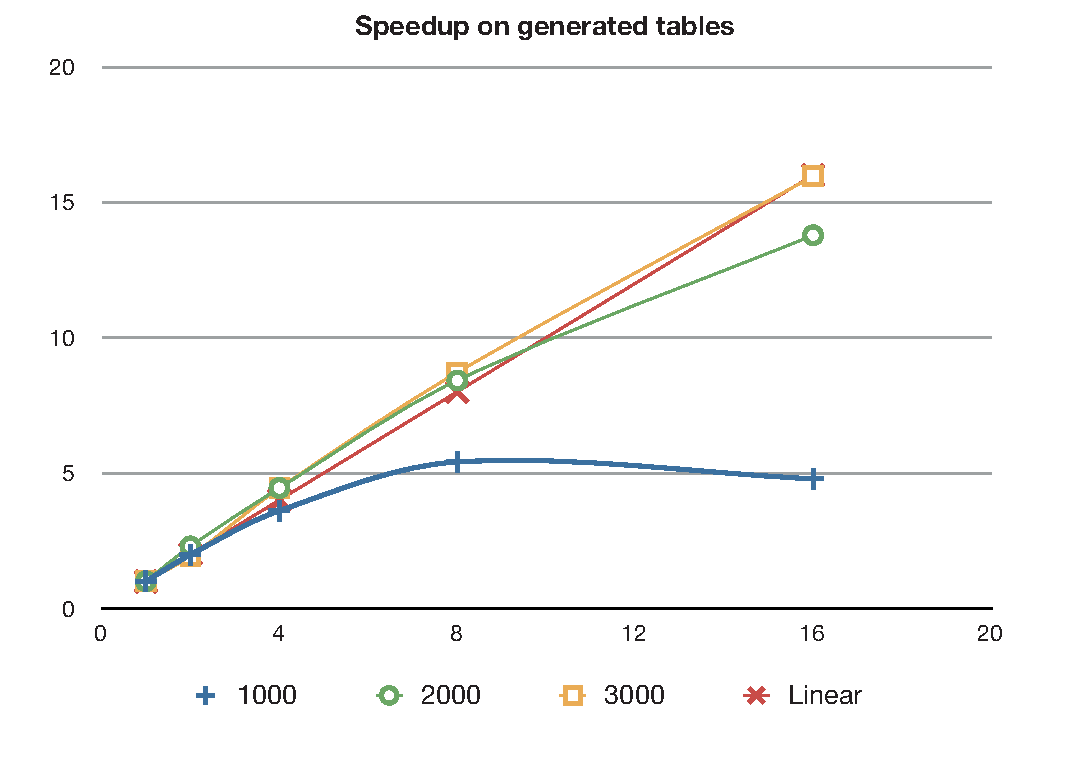
\includegraphics[scale=0.8]{figures/speedup.pdf}
\end{figure}

\end{document}
